\newpage
\section{Appendix}
\label{sxn:appendix}



\begin{table}[t]
\small
\begin{center}
\begin{tabular}{|p{1in}|c|c|c|c|c|c|c|}
\hline
Architecture 
 & Model
 & Top 1 Error \\
 \hline
 DenseNet & densenet121 & 25.57 & \\
& densenet161 & 22.86 & \\
& densenet169 & 24.4 & \\
& densenet201 & 23.1 & \\\hline
DPN & dpn68 & 24.17 & \\
& dpn98 & 20.81 & \\
& dpn131 & 20.54 & \\
\hline
MeNet & menet108\_8x1\_g3 & 43.92 & \\
& menet128\_8x1\_g4 & 43.95 & \\
& menet228\_12x1\_g3 & 33.57 & \\
& menet256\_12x1\_g4 & 33.41 & \\
& menet348\_12x1\_g3 & 30.1 & \\
& menet352\_12x1\_g8 & 33.31 & \\
& menet456\_24x1\_g3 & 28.4 & \\
\hline
MobileNet & mobilenet\_wd4 & 46.26 & \\
& mobilenet\_wd2 & 36.3 & \\
& mobilenet\_w3d4 & 33.54 & \\
& mobilenet\_w1 & 29.86 & \\
\hline
MobileNetV2 & mobilenetv2\_wd4 & 49.72 & \\
& mobilenetv2\_wd2 & 36.54 & \\
& mobilenetv2\_w3d4 & 31.89 & \\
& mobilenetv2\_w1 & 29.31 & \\
\hline
FDMobileNet & fdmobilenet\_wd4 & 55.77 & \\
& fdmobilenet\_wd2 & 43.85 & \\
& fdmobilenet\_w1 & 34.7 & \\
\hline
SE-ResNet & seresnet50 & 22.47 & \\
& seresnet101 & 21.88 & \\
& seresnet152 & 21.48 & \\
\hline
SE-ResNeXt & seresnext50\_32x4d & 21.0 & \\
& seresnext101\_32x4d & 19.96 & \\
\hline
ShuffleNet & shufflenetv2\_wd2 & 41.48 & \\
& shufflenetv2\_w1 & 34.39 & \\
\hline
\end{tabular}
\end{center}
\caption{Even more pretrained DNN models.  }
\label{table:models}
\end{table}


\begin{figure}[!htb]
    \centering
    \subfigure[DenseNet]{
        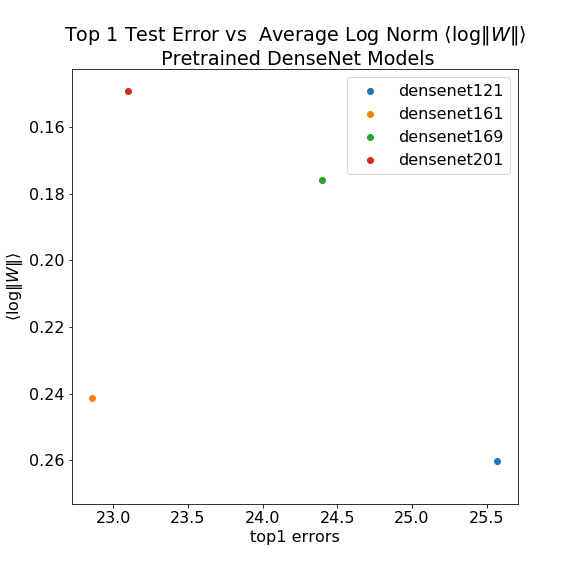
\includegraphics[scale=0.25]{img/DenseNet_top1-lognorms.png} 
        \label{fig:densenet-small}
    }
    \subfigure[DPN]{
        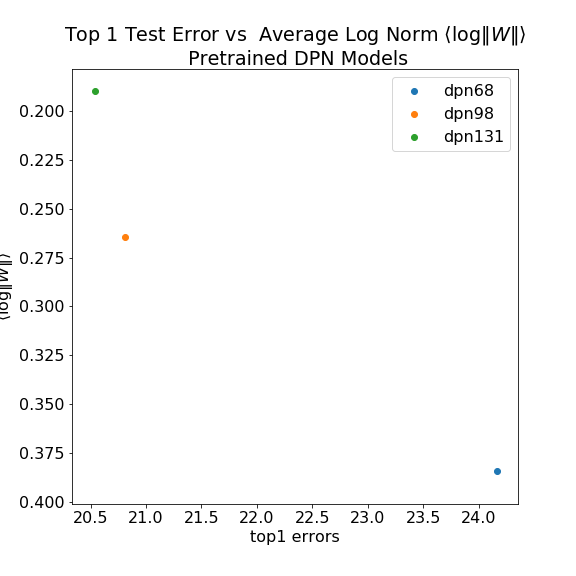
\includegraphics[scale=0.25]{img/DPN_top1-lognorms.png} 
        \label{fig:dpn-net}
    }
     \subfigure[ShuffleNet]{
        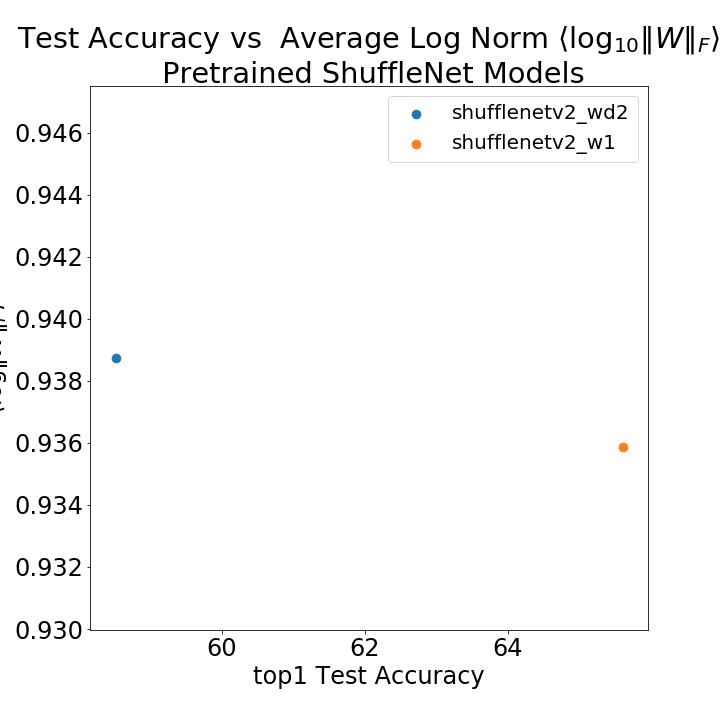
\includegraphics[scale=0.25]{img/ShuffleNet_top1-lognorms.png} 
        \label{fig:shufflenet-small}
    }
    \subfigure[MeNet]{
        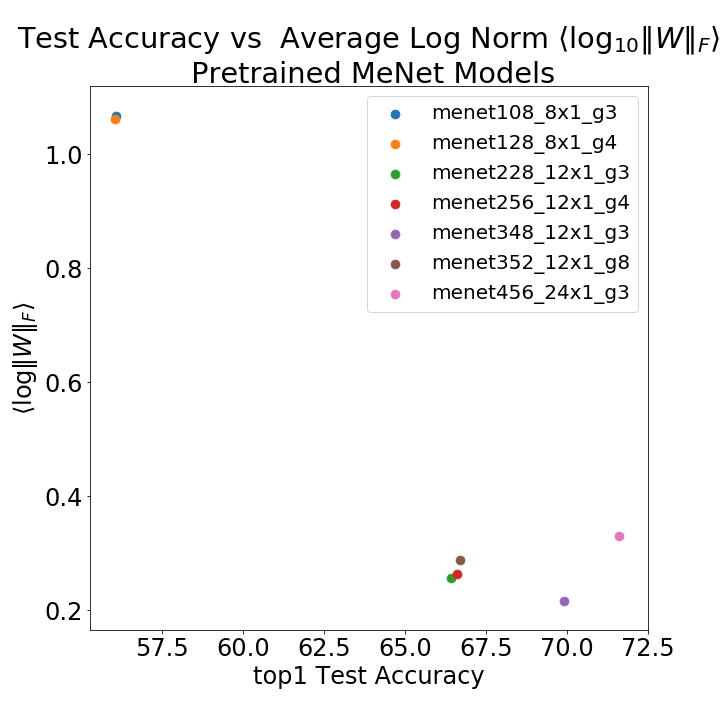
\includegraphics[scale=0.25]{img/MeNet_top1-lognorms.png} 
        \label{fig:menet-net}
    }
        \caption{DenseNet, DPN, ShuffleNet, MeNet}
    \label{fig:more-examples1}
\end{figure}





\begin{figure}[!htb]
 \centering
   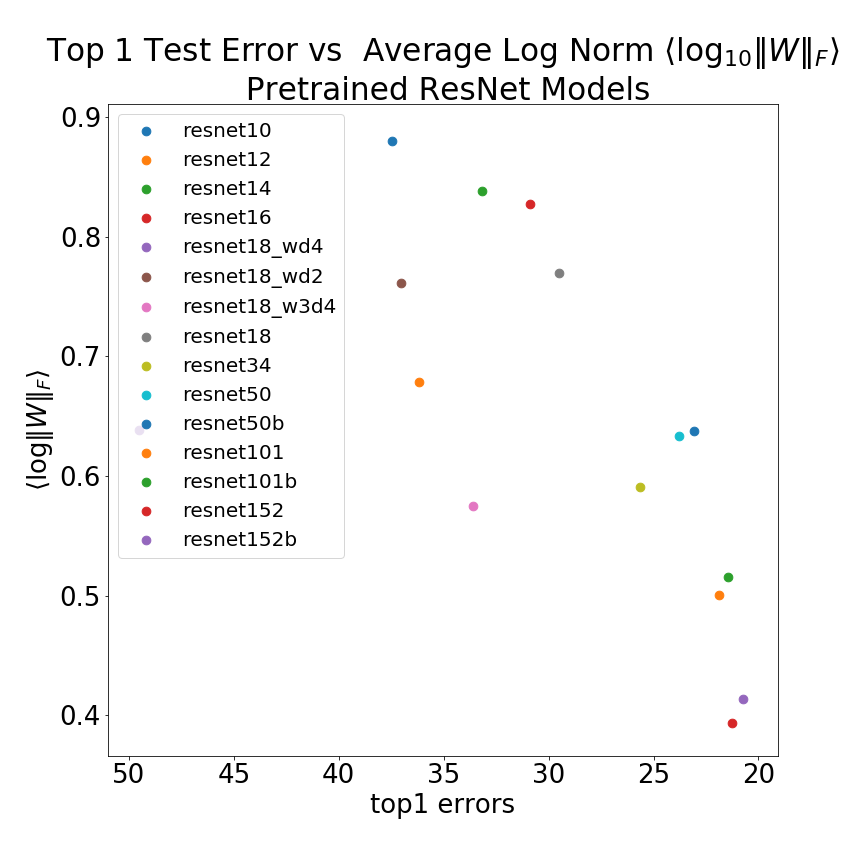
\includegraphics[scale=0.40]{img/ResNet_top1-lognorms.png}
   \caption{
Pretrained ResNet models available in OSMR package}
  \label{fig:resnet}
\end{figure}





\begin{table}[t]
\small
\begin{center}
\begin{tabular}{|p{1in}|c|c|c|c|c|c|c|}
\hline
Architecture 
 & Model
 & Top 1 Error & $\hat{\alpha}$ \\
\hline
ResNet (small)  & resnet10 & 37.46 & \\
& resnet12 & 36.18 & \\
& resnet14 & 33.17 & \\
& resnet16 & 30.9 & \\
& resnet18 & 29.52 & \\
& resnet34 & 25.66 & \\
& resnet50 & 23.79 & \\
\hline
CondenseNet & condensenet74\_c4\_g4 & 26.25 & \\
& condensenet74\_c8\_g8 & 28.93 & \\
\hline
\end{tabular}
\end{center}
\caption{Counter Examples}
\label{table:models}
\end{table}



\begin{figure}[!htb]
    \centering
    \subfigure[MobileNet]{
        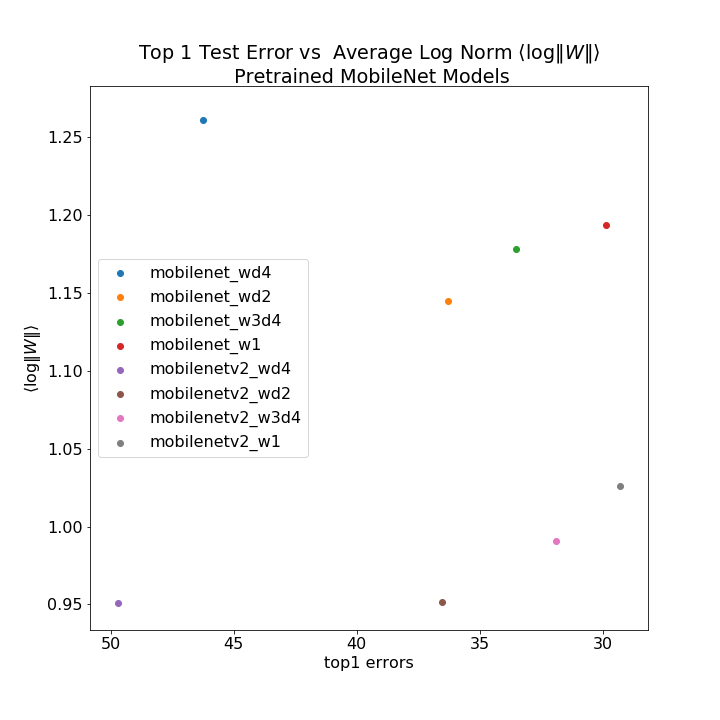
\includegraphics[scale=0.25]{img/MobileNet_top1-lognorms.png} 
        \label{fig:resnet-small}
    }
    \subfigure[CondenseNet]{
        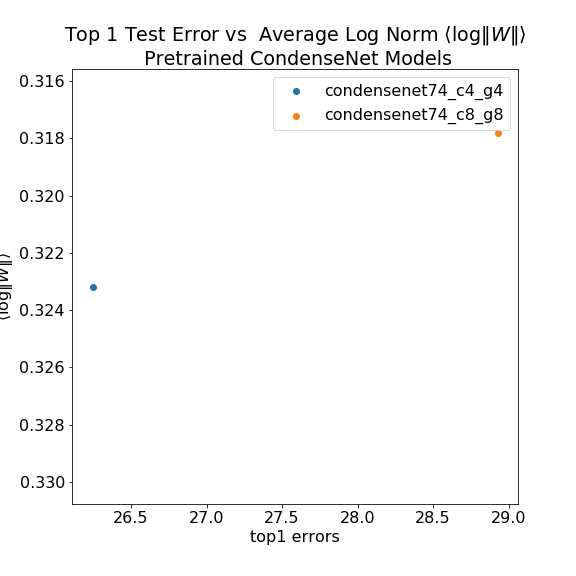
\includegraphics[scale=0.25]{img/CondenseNet_top1-lognorms.png} 
        \label{fig:condense-net}
    }
        \caption{CounterExamples}
    \label{fig:counter-examples}
\end{figure}



